\documentclass[12pt,ngerman]{beamer}

\usepackage[utf8]{inputenc}
\usepackage[T1]{fontenc}
\usepackage{booktabs}
\usepackage{babel}
\usepackage{graphicx}
\usepackage{csquotes}
\usepackage{xcolor}
\usepackage{listings}
\usepackage{mdframed}
\usepackage{tikz}

\definecolor{hellgelb}{rgb}{1,1,0.8}
\definecolor{lightgelb}{rgb}{1,1,0.8}
\definecolor{colKeys}{rgb}{0,0,1}
\definecolor{colIdentifier}{rgb}{0,0,0}
\definecolor{colComments}{rgb}{1,0,0}
\definecolor{colString}{rgb}{0,0.5,0}

\newcounter{Aufgabe}
\setcounter{Aufgabe}{1}

\usepackage{mdframed}

\newmdenv [linecolor=blue, leftmargin=0.1\textwidth,rightmargin=0.1\textwidth]{infobox}

% Venn Diagrams
% Definition of circles
\def\firstcircle{(0,0) circle (2cm)}
\def\secondcircle{(0:3cm) circle (2cm)}

\colorlet{circle edge}{blue!50}
\colorlet{circle area}{blue!20}

\tikzset{filled/.style={fill=circle area, draw=circle edge, thick},
    outline/.style={draw=circle edge, thick}}

%%% end venn

\newcommand{\Aufgabe}{Aufgabe~%
\stepcounter{Aufgabe}%
\theAufgabe%
}

\usepackage{textcomp}
\lstset{%
	language=Python,%	
    float=hbp,%
    basicstyle=\ttfamily\footnotesize, %
    identifierstyle=\color{colIdentifier}, %
    keywordstyle=\color{colKeys}, %
    stringstyle=\color{colString}, %
    commentstyle=\color{colComments}, %
    alsoletter={\_},
	language= {Python},%
    columns=flexible, %
    tabsize=2, %
    morekeywords={read_csv,system,startfile,close,read,isoformat,now,to_datetime,merge,to_excel,join,concat,pairplot,vq,kmeans,savefig,Series,axis,DataFrame,index,to_frame,loc,iloc,idx,mean,describe,std,count,},%
    frame=single, %
    extendedchars=true, %
    showspaces=false, %
    showstringspaces=false, %
    numbers=left, %
    numberstyle=\tiny, %
    upquote=true,
    breaklines=true, %
    backgroundcolor=\color{yellow!15}, %
    breakautoindent=true, %
    captionpos=b%
}


\lstset{literate=%
    {Ö}{{\"O}}1
    {Ä}{{\"A}}1
    {Ü}{{\"U}}1
    {ß}{{\ss}}1
    {ü}{{\"u}}1
    {ä}{{\"a}}1
    {ö}{{\"o}}1
    {~}{{\textasciitilde}}1
}

\newcommand{\pp}[1]{\lstinline[language={Python}]{#1}}


\author{Dr. Uwe Ziegenhagen}
\title{Python \& \LaTeX}
\subtitle{Dante e.\,V. Frühjahrstagung 2017}
\date{22. März 2017}

\begin{document}

\begin{frame}

\begin{itemize}
	\item Wer aktiv mitmachen möchte, setzt sich bitte nach vorn.
	\item Einen USB-Stick mit Anaconda hab ich dabei
	\item Alle Folien \& Beispiele auch auf dem Stick
	\item oder unter \url{https://github.com/UweZiegenhagen/PythonAndLaTeX}
	\end{itemize}
\end{frame}

\begin{frame}

\maketitle

\end{frame}


\begin{frame}
\frametitle{Überblick}
\framesubtitle{Was machen wir heute?}

\begin{itemize}
\item Python Grundlagen
\item Python in \LaTeX\ Dokumenten
\item Erzeugung von \LaTeX\ Dokumenten
\end{itemize}
\end{frame}


\begin{frame}
\frametitle{Voraussetzungen}
\framesubtitle{Was wird benötigt}

\begin{itemize}
\item Aktuelle \TeX\ Installation (\TeX~Live 2016)
\item Python3 Installation, vorzugsweise Anaconda
\item Pakete:
\begin{itemize}
	\item numpy
	\item jinja2
	\item pandas
\end{itemize}
\item Diese Folien und Code-Beispiele unter: 
\end{itemize}

\url{https://github.com/UweZiegenhagen/PythonAndLaTeX}

\end{frame}


\begin{frame}
\frametitle{\enquote{Scientific Python} Distributionen}
\framesubtitle{~}

\begin{itemize}
	\item Linux/MacOS X kommen mit Python, aber nicht SciPy
	\item Manuell nachinstallieren oder \enquote{echte} Installation
	\item Meine Empfehlung: Anaconda
\begin{itemize}
	\item Anaconda (\url{https://www.continuum.io/downloads})
	\item WinPython (\url{https://winpython.github.io})
\end{itemize}
	\end{itemize}
	
\begin{center} % left bottom right top
\fbox{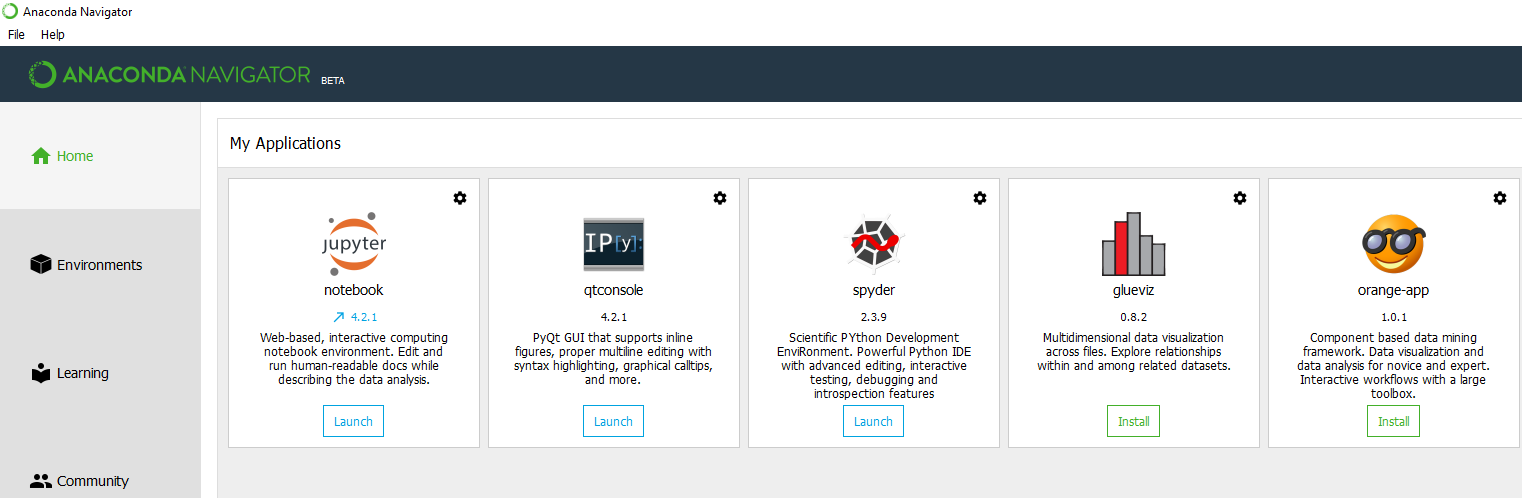
\includegraphics[width=\textwidth]{Bilder/anaconda}}
\end{center}	
\end{frame}

\begin{frame}
\frametitle{Das SciPy Framework}
\framesubtitle{~}

SciPy-Distributionen enthalten:

\begin{description}
\item[NumPy] Matrizen, Vektoren, Algorithmen
\item[IPython] Matlab/Mathematica-ähnliche Umgebung
\item[Matplotlib] Wiss. Grafik, Basis für die \texttt{seaborn} Bibliothek
\item[SymPy] Symbolische Mathematik
\item [\ldots] etc,\,etc.
\end{description}
\end{frame}


\begin{frame}[containsverbatim]
\frametitle{Testen der Installation}

\begin{itemize}
	\item Funktionieren die folgenden Befehle?
\end{itemize}

\begin{lstlisting}
import jinja2
import pandas
import numpy
\end{lstlisting}

Wenn ja, dann gut, wenn nein, dann 

\begin{itemize}
	\item entweder Anaconda installieren :-)
	\item oder mittels \texttt{pip} nachinstallieren :-(
\end{itemize}

\end{frame}

\begin{frame}
\frametitle{Anaconda Installation 1}

\begin{center}
\fbox{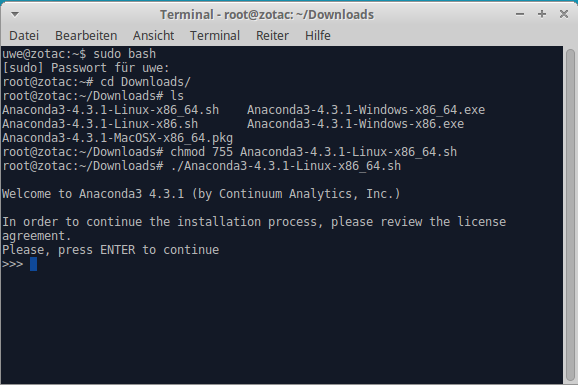
\includegraphics[width=0.8\textwidth]{Bilder/Anaconda-01}}
\end{center}

\end{frame}

\begin{frame}
\frametitle{Anaconda Installation 2}

\begin{center}
\fbox{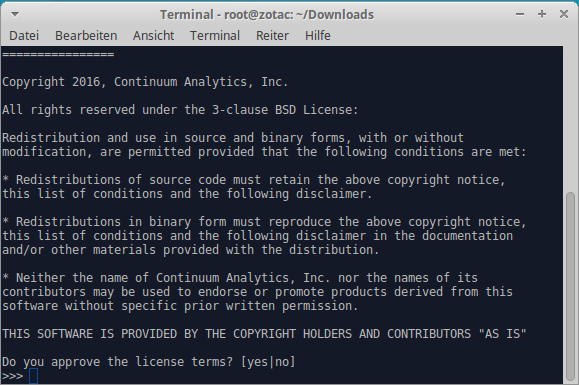
\includegraphics[width=0.8\textwidth]{Bilder/Anaconda-02}}
\end{center}

\end{frame}

\begin{frame}
\frametitle{Anaconda Installation 3}

\begin{center}
\fbox{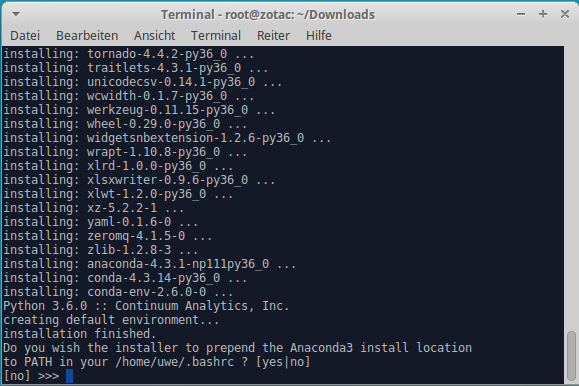
\includegraphics[width=0.8\textwidth]{Bilder/Anaconda-03}}
\end{center}

\end{frame}


\begin{frame}
\frametitle{Anaconda Installation 4}

\texttt{sudo conda update ----all}

\begin{center}
\fbox{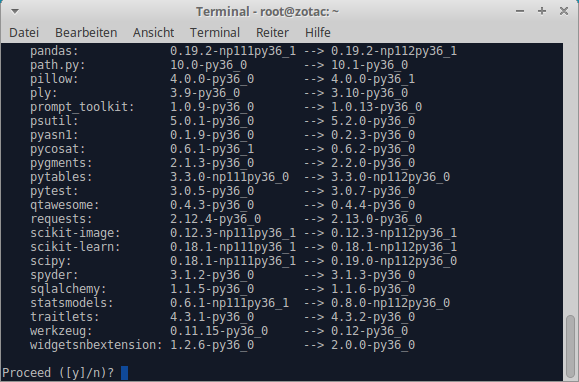
\includegraphics[width=0.8\textwidth]{Bilder/Anaconda-04}}
\end{center}

\end{frame}


\begin{frame}
\frametitle{Anaconda Installation 5}

Läuft\ldots

\begin{center}
\fbox{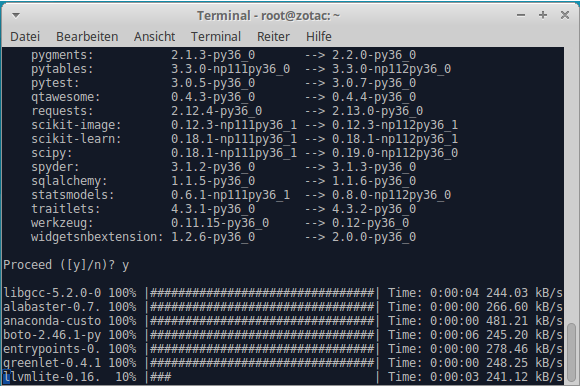
\includegraphics[width=0.8\textwidth]{Bilder/Anaconda-05}}
\end{center}

\end{frame}





\section{Python Grundlagen}

\begin{frame}
\frametitle{Python}
\framesubtitle{~}

\begin{itemize}
	\item Erfunden von Guido van Rossum (Niederlande)
	\item Fokus auf lesbaren und verständlichen Code
	\item umfangreiche Standard-Bibliothek $\Rightarrow$  \enquote{batteries included} 
	\item Mein erster Kontakt mit Python: Downloadskript für den Save.TV Online-VCR
	\item Python2 versus Python3 $\Rightarrow$ Python3
	\item Editor/IDE? Ich nutze Spyder3, auch empfehlenswert: Geany
	\item Python selbst liefert IDLE mit
\end{itemize}
\end{frame}

\begin{frame}[fragile]
\frametitle{\Aufgabe}
\framesubtitle{Python \enquote{Hello World}}

\begin{itemize}
	\item Editor der Wahl starten, folgende Befehle ausprobieren
\end{itemize}

\lstinputlisting[firstline=7,caption={Hello World in Python 3.x, sources/helloWorld.py}]{sources/helloWorld.py}

\end{frame}


\begin{frame}[fragile]
\frametitle{Strings, Listen und Tupel}
\framesubtitle{Strings}

\lstinputlisting[firstline=7,caption={Strings, sources/Strings.py}]{sources/Strings.py}

\end{frame}

\begin{frame}[fragile]
\frametitle{Strings, Listen und Tupel}
\framesubtitle{Stringfunktionen}

\lstinputlisting[firstline=7,caption={Strings, sources/Strings2.py}]{sources/Strings2.py}
\end{frame}


\begin{frame}[fragile]
\frametitle{Strings, Listen und Tupel}
\framesubtitle{Listen}

\begin{itemize}
	\item Index von $0$ bis $n-1$
	\item veränderbar
\end{itemize}

\lstinputlisting[firstline=8,caption={Listen, sources/Listen.py}]{sources/Listen.py}

\end{frame}


\begin{frame}[fragile]
\frametitle{Strings, Listen und Tupel}
\framesubtitle{Tupel}

\begin{itemize}
	\item ähnlich wie Listen
	\item Index von $0$ bis $n-1$
	\item nicht veränderbar, also \enquote{schreibgeschützt}
\end{itemize}


\lstinputlisting[firstline=7,caption={Tupel, sources/Tupel.py}]{sources/Tupel.py}
\end{frame}

\begin{frame}[fragile]
\frametitle{Dictionaries}
\framesubtitle{Key-Value Paare}

\begin{itemize}
	\item nicht veränderbar
\end{itemize}

\lstinputlisting[firstline=7,caption={Tupel, sources/Dictionaries.py}]{sources/Dictionaries.py}
\end{frame}

\section{Programmfluss}

\begin{frame}[fragile]
\frametitle{Flusssteuerung}
\framesubtitle{if/then}

\lstinputlisting[firstline=7,caption={if-then, sources/ifthen.py}]{sources/ifthen.py}

"condition"\ kann ein üblicher Boolean Ausdruck sein.

\end{frame}

\begin{frame}[fragile]
\frametitle{Flusssteuerung}
\framesubtitle{for}

\lstinputlisting[firstline=7,caption={for-Schleifen, sources/for.py}]{sources/for.py}

\end{frame}

\begin{frame}[fragile]
\frametitle{Flusssteuerung}
\framesubtitle{while}

\lstinputlisting[firstline=7,caption={while-Schleifen, sources/while.py}]{sources/while.py}

\end{frame}

\begin{frame}[fragile]
\frametitle{Funktionen}
\framesubtitle{~}

\lstinputlisting[firstline=7,caption={Definition von Funktionen, sources/Funktionen.py}]{sources/Funktionen.py}

\end{frame}


\begin{frame}[fragile]
\frametitle{Ein- und Ausgabe}
\framesubtitle{Kommandozeile}

\lstinputlisting[firstline=7,caption={Ein- und Ausgabe: Kommandozeile, sources/io.py}]{sources/io.py}

\end{frame}

\begin{frame}[fragile]
\frametitle{Ein- und Ausgabe}
\framesubtitle{Dateien lesen}

\lstinputlisting[firstline=7,caption={Ein- und Ausgabe: Dateien, sources/readWriteFile.py}]{sources/readWriteFile.py} 

\end{frame}


\begin{frame}[fragile]
\frametitle{Ein- und Ausgabe}
\framesubtitle{UTF8-Dateien lesen und schreiben}

\lstinputlisting[firstline=7,caption={UTF8, sources/readWriteUTF8.py}]{sources/readWriteUTF8.py} 

\end{frame}

\begin{frame}[fragile]
\frametitle{Andere wichtige Befehle}
\framesubtitle{Das \texttt{os} Modul}

\texttt{os} enthält verschiedenste Funktionen für den Umgang mit Dateien und Prozessen, für uns spannend:

\begin{itemize}
\item \lstinline{os.system(<Befehl>)} Führt externen Befehl aus
\item \lstinline{os.startfile(<Datei>)} Öffnet Datei mit der Standard-Applikation (nur unter Windows)
\end{itemize}
\end{frame}

\begin{frame}[fragile]
\frametitle{Aufgabe \theAufgabe}
\framesubtitle{Wir (lassen) rechnen\ldots}

\begin{itemize}
\item Wir erzeugen Rechenaufgaben für Kinder
\item links die Aufgabe, rechts die Lösung
\item Aufgaben randomisiert (\texttt{random} Modul)
\item Datei automatisch übersetzen und ausführen
\item Tipp für die Schriftart: TeX Gyre Schola, \verb|\usepackage{tgschola}|
\end{itemize}
\end{frame}

\begin{frame}[fragile]
\frametitle{Lösung}
\framesubtitle{Teil 1}

\lstinputlisting[firstline=7,lastline=12,caption={Rechnen Teil 1, sources/Aufgaben.py}]{sources/Aufgaben.py} 

\end{frame}

\begin{frame}[fragile]
\frametitle{Lösung}
\framesubtitle{Teil 2}

\lstinputlisting[firstline=14,lastline=24,caption={Rechnen Teil 2, sources/Aufgaben.py}]{sources/Aufgaben.py} 

\end{frame}

\begin{frame}[fragile]
\frametitle{Lösung}
\framesubtitle{Teil 3}

\lstinputlisting[firstline=26,lastline=38,caption={Rechnen Teil 3, sources/Aufgaben.py}]{sources/Aufgaben.py} 

\end{frame}

\section{Python in \LaTeX-Dokumenten}

\begin{frame}
\frametitle{Python und \LaTeX\ verbinden}
\framesubtitle{~}

Q: Wie kann man \LaTeX~ und Python in nur einem Dokument verwalten?

A: Literate programming\footnote{WEB, CWEB, NOWEB, SWEAVE, knitR}

\begin{itemize}
\item etwas \enquote{Selbstgestricktes}
\item Python\TeX\ von Ge­of­frey M. Poore \url{https://www.ctan.org/pkg/pythontex}
\end{itemize}
\end{frame}

\begin{frame}
\frametitle{Python im \LaTeX-Lauf}

\begin{center}
\fbox{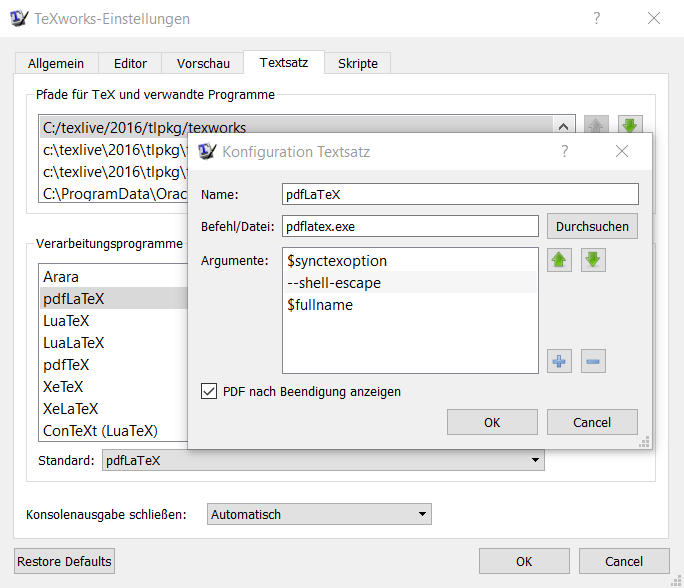
\includegraphics[width=0.8\textwidth]{Bilder/shellescape}}
\end{center}

\end{frame}


\begin{frame}[fragile]
\frametitle{Python im \LaTeX-Lauf}

\begin{lstlisting}[basicstyle={\ttfamily\footnotesize},language={TeX},morekeywords={makeatletter,endVerbatimOut,typeout,lstinputlisting,makeatother,VerbatimOut,footnotesize}]
\makeatletter
\newenvironment{pycode}[1]%
  {\xdef\d@tn@me{#1}\xdef\r@ncmd{python #1.py > #1.plog}%
  \typeout{Writing file #1}\VerbatimOut{#1.py}% 
  }
  {\endVerbatimOut %
 \toks0{\immediate\write18}%
 \expandafter\toks\expandafter1\expandafter{\r@ncmd}%
 \edef\d@r@ncmd{\the\toks0{\the\toks1}}\d@r@ncmd %
 \lstinputlisting[language={Python},label=listing:\d@tn@me,basicstyle={\ttfamily\footnotesize}]{\d@tn@me.py}%
 \lstinputlisting[basicstyle={\ttfamily\footnotesize}]{\d@tn@me.plog}%
}
\makeatother
\end{lstlisting}
\end{frame}

\begin{frame}
\frametitle{Python im \LaTeX-Lauf}
\framesubtitle{~}

Beispiele unter \texttt{/sources}, leicht anpassbar

\begin{description}
\item [pycode-mini.tex] einspaltig s/w
\item [pycode.tex] einspaltig, farbig hinterlegt
\item [pycode-beamer.tex] für Folien, zweispaltig
\end{description}
\end{frame}



\begin{frame}
\frametitle{Python\TeX}

\begin{itemize}
\item \enquote{PythonTeX} Paket von Ge­of­frey M. Poore
\item Paket in Version 0.15 auf CTAN, auch in \newline \TeX~Live 2016 enthalten
\item unter Windows \texttt{pythontex.exe}
\item stellt mehrere Befehle und Umgebungen bereit
\item Syntax-Highlighting via \texttt{pygments}
\item komplexer als die \enquote{Eigenbau-Lösung} 
\item Workflow
\begin{itemize}
	\item Kompiliere Dokument mit \texttt{*latex}
	\item Lass \texttt{pythontex.exe}/\texttt{pythontex.py} laufen
	\item Kompiliere Dokument wieder mit \texttt{*latex}
\end{itemize}

\end{itemize}
\end{frame}


\begin{frame}[fragile]
\frametitle{Arara-Regel}

Hilfreich dabei: eigene Arara-Regel

\begin{itemize}
	\item Was ist Arara?
	\item \url{texwelt.de/wissen/fragen/8764/was-ist-arara}
	\item ablegen unter \texttt{C:/texlive/2016/texmf-dist/ scripts/arara/rules} oder im lokalen texmf-Tree
\end{itemize}

\lstinputlisting[caption={UTF8, sources/pythontex.yaml},basicstyle=\ttfamily\scriptsize]{sources/pythontex.yaml}
\end{frame}

\begin{frame}[fragile]
\frametitle{Python\TeX}

Befehle

\begin{itemize}
\item \verb|\py{}|  für Code, der einen String zurückliefert
\item \verb|\pyc{}|  für Code, der nur ausgeführt wird
\item \verb|\pys{}|  mit Substitution
\item \verb|\pyv{}|  für Code, der nur gesetzt wird
\item \verb|\pyb{}|  für Ausführung und Satz der Ergebnisse
\end{itemize}

Umgebungen

\begin{description}
\item[pycode] wie \texttt{pyc}
\item[pysub] wie \texttt{pys}
\item[pyverbatim] wie \texttt{pyv}
\item[pyblock] wie \texttt{pyb}
\item[pyconsole] simuliert eine Python-Konsole
\end{description}

\end{frame}

\begin{frame}
\frametitle{Python\TeX}
\framesubtitle{Beispiele aus der Python\TeX-Galerie}

Alle Beispiele unter \texttt{/sources}

\begin{description}
\item[pythontex-01.tex] \enquote{Hallo Welt}
\item[pythontex-02.tex] Formatstring
\item[pythontex-03.tex] Substitution
\item[pythontex-04.tex] Unicode und Pyconsole
\item[pythontex-05.tex] Pyconsole Evaluation
\item[pythontex-06.tex] SymPy
\end{description}

\end{frame}

\begin{frame}[fragile]
\frametitle{Eigenes Beispiel}
\framesubtitle{Erzeugung einer Verteilungstabelle}

\lstinputlisting[basicstyle=\scriptsize,firstline=20,lastline=38,caption={Normalverteilung, sources/pythontex-07.tex}]{sources/pythontex-07.tex} 

\end{frame}


\begin{frame}
\frametitle{Daten verarbeiten}
\framesubtitle{Die wunderbare Welt von \texttt{pandas}}

\begin{itemize}
\item mein \enquote{täglich Brot}: Datenbestände zwischen Banksystemen abgleichen 
\item \enquote{pandas is an open source, BSD-licensed library providing high-performance, easy-to-use data structures and data analysis tools for the Python programming language.}\footnote{Source: \url{pandas.pydata.org}}
\item Initiiert 2008 durch Wes McKinney von AQR Capital Management für hoch-performante quantitative Analyse
\item Wesentliche Teile in C/Cython implementiert
\item  Current version is 0.19
\end{itemize}
\end{frame}

\section{Data Handling with \texttt{pandas}}

\begin{frame}
\frametitle{Series und DataFrames}

\begin{itemize}
	\item central data structures in \texttt{pandas}
\end{itemize}\vspace*{1em}

\begin{figure}
\begin{center}
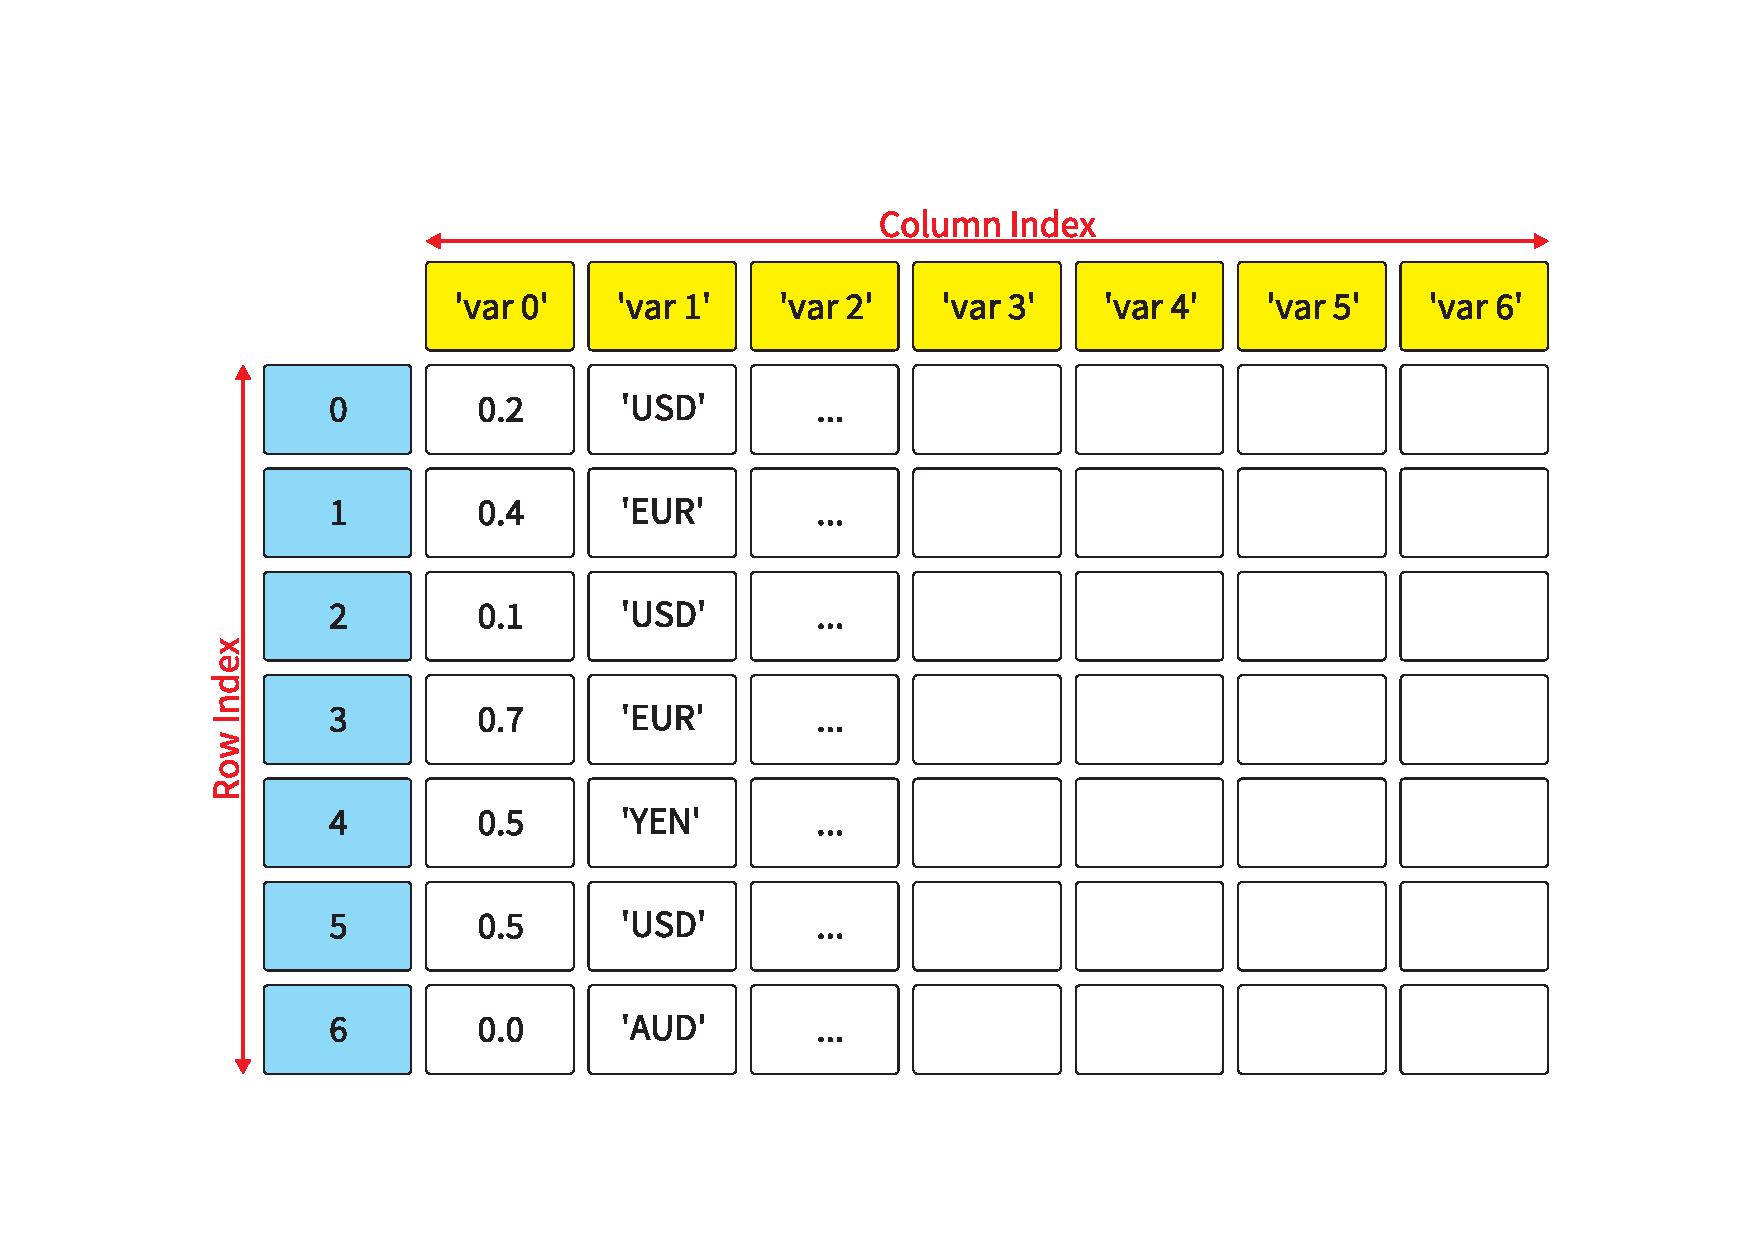
\includegraphics[trim=50mm 55mm 45mm 55mm,width=0.8\textwidth]{Bilder/SeriesFrames.pdf}
\end{center}
\end{figure}
\end{frame}


\begin{frame}
\frametitle{Daten lesen}
\framesubtitle{~}

\begin{center}
\begin{tabular}{ll} \toprule
Command & Description \\ \midrule
read\textunderscore pickle &lies Pickle objects \\
read\textunderscore table & für Tabellenformate \\
read\textunderscore csv & Comma-Separated Values  \\
read\textunderscore fwf & für fixed-width Formate\\
read\textunderscore clipboard & lies aus der Zwischenablage \\
read\textunderscore excel & lies Excel-Dateien\\ \bottomrule
\end{tabular}\vspace*{-0.35em}
\end{center}

andere Befehle für HTML, JSON, HDF5, \ldots
\end{frame}

\begin{frame}[fragile]
\frametitle{CSV-Formate lesen}
\framesubtitle{~}

\begin{itemize}
\item CSV $\not=$ CSV
\begin{itemize}
	\item Spaltentrenner
	\item Dezimaltrenner
	\item Encoding
\end{itemize}
\item \url{http://pandas.pydata.org/pandas-docs/stable/generated/pandas.read_csv.html}
\begin{description}
\item[sep] Spaltentrenner
\item[thousands] Tausender-Trenner
\item[encoding] hoffentlich UTF8
\item [decimal]  Dezimaltrenner
\item [converters] converters=\{'A': str\} für Konvertierung
\end{description}
\end{itemize}
\end{frame}

\begin{frame}
\frametitle{Excel lesen}

\begin{itemize}
\item \pp{pd.read_excel()} für XLSX-Dateien
\item Dokumentation: \url{http://pandas.pydata.org/pandas-docs/stable/generated/pandas.read_excel.html}
\item Export nach Excel: \pp{pd.to_excel()} function
\item Hinweise:
\begin{itemize}
	\item Excel-export langsamer als CSV-Export
	\item \enquote{Schickes} Excel ist aufwändiger
	\item Excel/Office kann auch gut per COM gesteuert werden
\end{itemize}
\end{itemize}
\end{frame}

\begin{frame}[fragile]
\frametitle{DataFrames abfragen}
\framesubtitle{Grundlegende Daten}

\begin{lstlisting}[language={Python}]
customers = pd.read_excel('Northwind.xlsx',
                          sheetname = 'Customers')

print(len(customers))     # Zeilenzahl
print(customers.head()) # die ersten 5 Zeilen
print(customers.tail())   # die letzten 5 Zeilen
print(list(customers))    # die Spaltennamen
\end{lstlisting}
\end{frame}

\begin{frame}[fragile]
\frametitle{Pandas Dataframe Operationen}
\framesubtitle{Auswahl und Filterung I}

\begin{itemize}
	\item pandas hat clevere  Funktionen zur Datenauswahl
\end{itemize}

\begin{itemize}
\item Wähle bestimmte Spalten aus

\pp{df = df[['colA', 'colB']]}

\item Wähle nur die ersten zwei Zeilen (Index beginnt mit 0)

\pp{df.iloc[:1]}

\item Wähle die Zeilen, in denen \texttt{ColA} > 50

\pp{df[df['colA'] > 50]}
\end{itemize}
\end{frame}

\begin{frame}[fragile]
\frametitle{Pandas Dataframe Operationen}
\framesubtitle{Auswahl und Filterung II}

\begin{itemize}
\item Wähle die Zeilen, in denen \texttt{colA} größer 50 und kleiner 500

\pp{df[(df['colA'] > 50) | (df['colA'] < 500)]}

\item Wähle die Zeilen, in denen \texttt{colA} nicht \enquote{HelloWorld} ist

\pp{df[~(df['colA'] == 'HelloWorld')]}

\item Wähle die Zeilen, in denen 'b' 'A' oder 'B' ist

\pp{df = df[ (df['b'] == 'A') | (df['b'] == 'I')]}

\item Alternative dazu via \pp{isin()}

\pp{df = df[df['b'].isin(['A','I'])]}

\item oder das Gegenstück dazu

\pp{df = df[~df['b'].isin(['A','I'])]}

\end{itemize}
\end{frame}


\begin{frame}[fragile]
\frametitle{Pandas Dataframe Operationen}
\framesubtitle{Merge}

\begin{itemize}
\item \texttt{merge()} join wie in SQL
\item nützlich, um Datensätze zu verbinden
\item Unterstützt werden
\begin{itemize}
	\item Left
	\item Right
	\item Inner
	\item Full Outer
\end{itemize}
\end{itemize}

\end{frame}

\begin{frame}[fragile]
\frametitle{Pandas Dataframe Operationen}
\framesubtitle{Merging}

\begin{itemize}
	\item Optionen für \texttt{merge()}
\end{itemize}

\begin{lstlisting}
leftDataFrame.merge(rightDataFrame, how='inner', 
on=None, left_on=None, right_on=None, left_index=False, 
right_index=False, sort=False, suffixes=('_x', '_y'), 
copy=True, indicator=False)
\end{lstlisting}

\begin{enumerate}
\item Definiere den anderen Datensatz
\item Definiere, wie verbunden werden soll
\item Definiere die Schlüsselspalten
\end{enumerate}

\end{frame}


\begin{frame}
\frametitle{Merging}
\framesubtitle{Inner Join}

\begin{itemize}
\item Alle Daten, die in A und B sind
\end{itemize}

\begin{center}
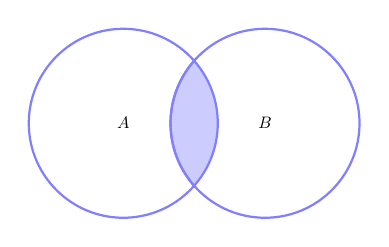
\begin{tikzpicture}[scale=0.6, every node/.style={scale=0.6}]
    \begin{scope}
        \clip \firstcircle;
        \fill[filled] \secondcircle;
    \end{scope}
    \draw[outline] \firstcircle node {$A$};
    \draw[outline] \secondcircle node {$B$};
    %\node[anchor=south] at (current bounding box.north) {$A \cap B$};
\end{tikzpicture}
\end{center}

{\footnotesize
\begin{columns}
\begin{column}{0.3\textwidth}
left \\
\begin{tabular}{c|cc} \toprule
   & A  &  Key \\ \midrule
0 & A0 &  K0 \\
1 & A1 &  K1 \\ 
2 & A2 &  K2 \\
3 & A3 &  \textcolor{red}{K4} \\ \bottomrule
\end{tabular}
\end{column}
\begin{column}{0.3\textwidth}
right \\
\begin{tabular}{c|cc} \toprule
   &  B   & Key \\ \midrule
0 &  B0 & K0 \\
1 &  B1 & K1 \\ 
2 &  B2 & K2 \\
3 &  C3 & \textcolor{red}{K5} \\ \bottomrule
\end{tabular}\end{column}
\begin{column}{0.3\textwidth}
merged \\
\begin{tabular}{c|ccc} \toprule
   & A  & B   & Key \\ \midrule
0 & A0 & B0 & K0 \\
1 & A1 & B1 & K1 \\ 
2 & A2 & B2 & K2 \\ \bottomrule
\end{tabular} \\
\vspace*{1.5em}
\end{column}
\end{columns}}


\end{frame}

\begin{frame}
\frametitle{Merging}
\framesubtitle{Left Join}

\begin{itemize}
\item Alle Daten, die in A sind, mit passenden Daten aus B
\end{itemize}

\begin{center}
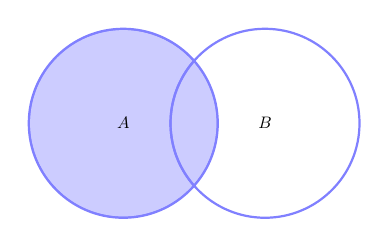
\begin{tikzpicture}[scale=0.6, every node/.style={scale=0.6}]
    \begin{scope}
        \clip \firstcircle;
        \draw[filled] \firstcircle node {$A$}
                                     \secondcircle;
    \end{scope}
    \draw[outline] \firstcircle
                   \secondcircle node {$B$};
    %\node[anchor=south] at (current bounding box.north) {$A - B$};
\end{tikzpicture}
\end{center}

{\footnotesize
\begin{columns}
\begin{column}{0.3\textwidth}
left \\
\begin{tabular}{c|cc} \toprule
   & A  &  Key \\ \midrule
0 & A0 &  K0 \\
1 & A1 &  K1 \\ 
2 & A2 &  K2 \\
3 & A3 &  \textcolor{red}{K4} \\ \bottomrule
\end{tabular}
\end{column}
\begin{column}{0.3\textwidth}
right \\
\begin{tabular}{c|cc} \toprule
   &  B   & Key \\ \midrule
0 &  B0 & K0 \\
1 &  B1 & K1 \\ 
2 &  B2 & K2 \\
3 &  C3 & \textcolor{red}{K5} \\ \bottomrule
\end{tabular}\end{column}
\begin{column}{0.3\textwidth}
merged \\
\begin{tabular}{c|ccc} \toprule
   & A  & B   & Key \\ \midrule
0 & A0 & B0 & K0 \\
1 & A1 & B1 & K1 \\ 
2 & A2 & B2 & K2 \\ \bottomrule
3 & A3 & NaN & K4 \\ \bottomrule
\end{tabular} \\
\vspace*{0.4em}
\end{column}
\end{columns}}

\end{frame}

\begin{frame}
\frametitle{Merging}
\framesubtitle{Right Join}

\begin{itemize}
\item Alle Daten, die in B sind, mit passenden Daten aus A
\end{itemize}

\begin{center}
% Right Join
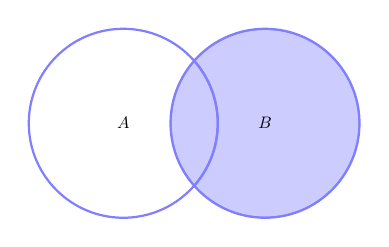
\begin{tikzpicture}[scale=0.6, every node/.style={scale=0.6}]
    \begin{scope}
        \clip \secondcircle;
        \draw[filled] \firstcircle \secondcircle node {$B$};
    \end{scope}
    \draw[outline] \firstcircle node {$A$}
                   \secondcircle;
    %\node[anchor=south] at (current bounding box.north) {$B - A$};
\end{tikzpicture}

\end{center}

{\footnotesize
\begin{columns}
\begin{column}{0.3\textwidth}
left \\
\begin{tabular}{c|cc} \toprule
   & A  &  Key \\ \midrule
0 & A0 &  K0 \\
1 & A1 &  K1 \\ 
2 & A2 &  K2 \\
3 & A3 &  \textcolor{red}{K4} \\ \bottomrule
\end{tabular}
\end{column}
\begin{column}{0.3\textwidth}
right \\
\begin{tabular}{c|cc} \toprule
   &  B   & Key \\ \midrule
0 &  B0 & K0 \\
1 &  B1 & K1 \\ 
2 &  B2 & K2 \\
3 &  C3 & \textcolor{red}{K5} \\ \bottomrule
\end{tabular}\end{column}
\begin{column}{0.3\textwidth}
merged \\
\begin{tabular}{c|ccc} \toprule
   & A  & B   & Key \\ \midrule
0 & A0 & B0 & K0 \\
1 & A1 & B1 & K1 \\ 
2 & A2 & B2 & K2 \\ 
3 & NaN & B3 & K5 \\ \bottomrule
\end{tabular} \\
\vspace*{0.4em}
\end{column}
\end{columns}}

\end{frame}


\begin{frame}
\frametitle{Merging}
\framesubtitle{Full Outer Join}

\begin{itemize}
\item Alle Daten, die in A oder B sind
\end{itemize}

\begin{center}
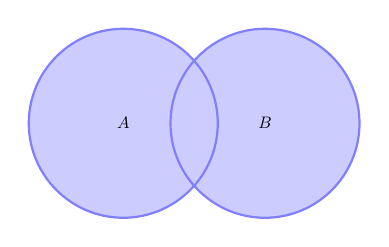
\begin{tikzpicture}[scale=0.6, every node/.style={scale=0.6}]
    \draw[filled] \firstcircle node {$A$}
                  \secondcircle node {$B$};
    %\node[anchor=south] at (current bounding box.north) {$A \cup B$};
\end{tikzpicture}
\end{center}

{\footnotesize
\begin{columns}
\begin{column}{0.3\textwidth}
left \\
\begin{tabular}{c|cc} \toprule
   & A  &  Key \\ \midrule
0 & A0 &  K0 \\
1 & A1 &  K1 \\ 
2 & A2 &  K2 \\
3 & A3 &  \textcolor{red}{K4} \\ \bottomrule
\end{tabular}
\vspace*{1.2em}
\end{column}
\begin{column}{0.27\textwidth}
right \\
\begin{tabular}{c|cc} \toprule
   &  B   & Key \\ \midrule
0 &  B0 & K0 \\
1 &  B1 & K1 \\ 
2 &  B2 & K2 \\
3 &  C3 & \textcolor{red}{K5} \\ \bottomrule
\end{tabular}
\vspace*{1.2em}
\end{column}
\begin{column}{0.3\textwidth}
merged \\
\begin{tabular}{c|ccc} \toprule
   & A  & B   & Key \\ \midrule
0 & A0 & B0 & K0 \\
1 & A1 & B1 & K1 \\ 
2 & A2 & B2 & K2 \\ 
3 & A3 & \textcolor{red}{NaN} & K4 \\ 
4 & \textcolor{red}{NaN} & B3 & K5 \\ \bottomrule
\end{tabular} \\
\vspace*{0.2em}
\end{column}
\end{columns}}



\end{frame}

\section{Jinja2}


\begin{frame}
\frametitle{jinja2}
\framesubtitle{Was ist eine \enquote{Template Engine}?}

\begin{infobox}
Jinja2 is a modern and designer-friendly templating language for Python, modelled after Django’s templates. It is fast, widely used and secure with the optional sandboxed template execution environment.
\end{infobox}

\begin{itemize}
	\item Vorlagen (aus Dateien, Datenbank, etc.)
	\item Liste von Variablen
	\item jinja2 ersetzt die Variablen durch Inhalte
	\item Erlaubt Trennung von Programmcode und Vorlage
\end{itemize}

\end{frame}

\begin{frame}[fragile]
\frametitle{jinja2}
\framesubtitle{Ein einfaches Beispiel (ohne \LaTeX)}

\lstinputlisting[,caption={Inhalt der Datei \enquote{test-min.txt}}]{sources/test-min.txt} 

\lstinputlisting[firstline=8,caption={UTF8, sources/jinja2-01.py}]{sources/jinja2-01.py} 

\end{frame}

\begin{frame}[fragile]
\frametitle{jinja2}
\framesubtitle{Eingebaute Schleifen}

\lstinputlisting[firstline=8,caption={UTF8, sources/jinja2-02.py}]{sources/jinja2-02.py} 

\end{frame}




\section{Beispiel}

\begin{frame}
\frametitle{Beispiel: Erstellung von Spendenbescheinigungen}
\framesubtitle{~}

\begin{itemize}
\item Schatzmeister des Kölner Dingfabrik e.V.
\item Manuelle Erstellung der Spendenbescheinigungen keine Option
\item Bis 2014: Python, MySQL, etc. (Siehe meinen Vortrag 2014 in Heidelberg)
\item Seither \texttt{pandas}, deutlich einfacher
\item Mehr dazu unter \url{http://uweziegenhagen.de/?p=3359}
\end{itemize}

Schauen wir uns das Beispiel unter \texttt{sources/Spendenquittungen} an

\end{frame}

\end{document}

